%Acá explicamos cómo extrajimos los datos, qué características tiene la muestra (muchos de los análisis/gráficos ya los hicimos), cómo la separamos, y qué análisis estadísticos estamos realizando (es la parte que nos falta)


\section{Extracción de Datos}

Para la recolección de tuits, primero se extrajo una cantidad de usuarios con información geográfica disponible con el fin de obtener todos sus tuits.
Los usuarios se buscaron por provincia de modo tal que haya una cantidad aproximadamente equitativa de cada una.
La búsqueda de los usuarios se hizo de la siguiente manera:

Por cada provincia de la Argentina, se extrajo las ubicaciones de cada uno de sus departamentos, de los partidos de la provincia de Buenos Aires y de las comunas de la Ciudad Autónoma de Buenos Aires. El conjunto de estas forman la subdivisión de segundo orden de la república Argentina. La lista de departamentos/partidos/comunas fue extraída a partir de los datos publicados del Censo Argentino del año 2010. Para extraer los tuits se utilizó la librería de \textit{python} llamada \textit{tweepy}.
De esta manera se recolectó aproximadamente 2000 usuarios por provincia, lo que resulta en 46000 usuarios argentinos. Sobre este conjunto de usuarios se buscaron los tuits. Se decidió no tener en cuenta los retuits dado que no son escritos por los usuarios sino que son una mera copia de otros tuits. 


\subsection{Búsquedas geolocalizadas}

La búsqueda geolocalizada es una herramienta que nos da la posibilidad de obtener tuits generados en un área geográfica particular. Para esto, primero intenta buscar tuits cuyas coordenadas sean las buscadas. En caso de no tener éxito, se busca aquellos tuits creados por usuarios que tienen en el campo \textit{location} de su perfil un lugar cuyo geocódigo coincida con el de sus coordenadas. Es decir, si se hace una búsqueda inversa de las coordenadas, devuelve el lugar de su perfil.

Una vez obtenida la lista de ubicaciones, se realizaron búsquedas por cada provincia con centro en las coordenadas de los departamentos de la misma y con un radio de 20 millas. Sobre el resultado de esta búsqueda, únicamente se seleccionaron los usuarios que tienen como campo \textit{location} al menos uno de los nombres de las ciudades de la provincia. 

En el gráfico de la figura \ref{fig:busqueda_usuarios} se muestran las ubicaciones de los usuarios.


\begin{figure}[!ht]\centering
  \begin{minipage}[t]{0.31\textwidth}
    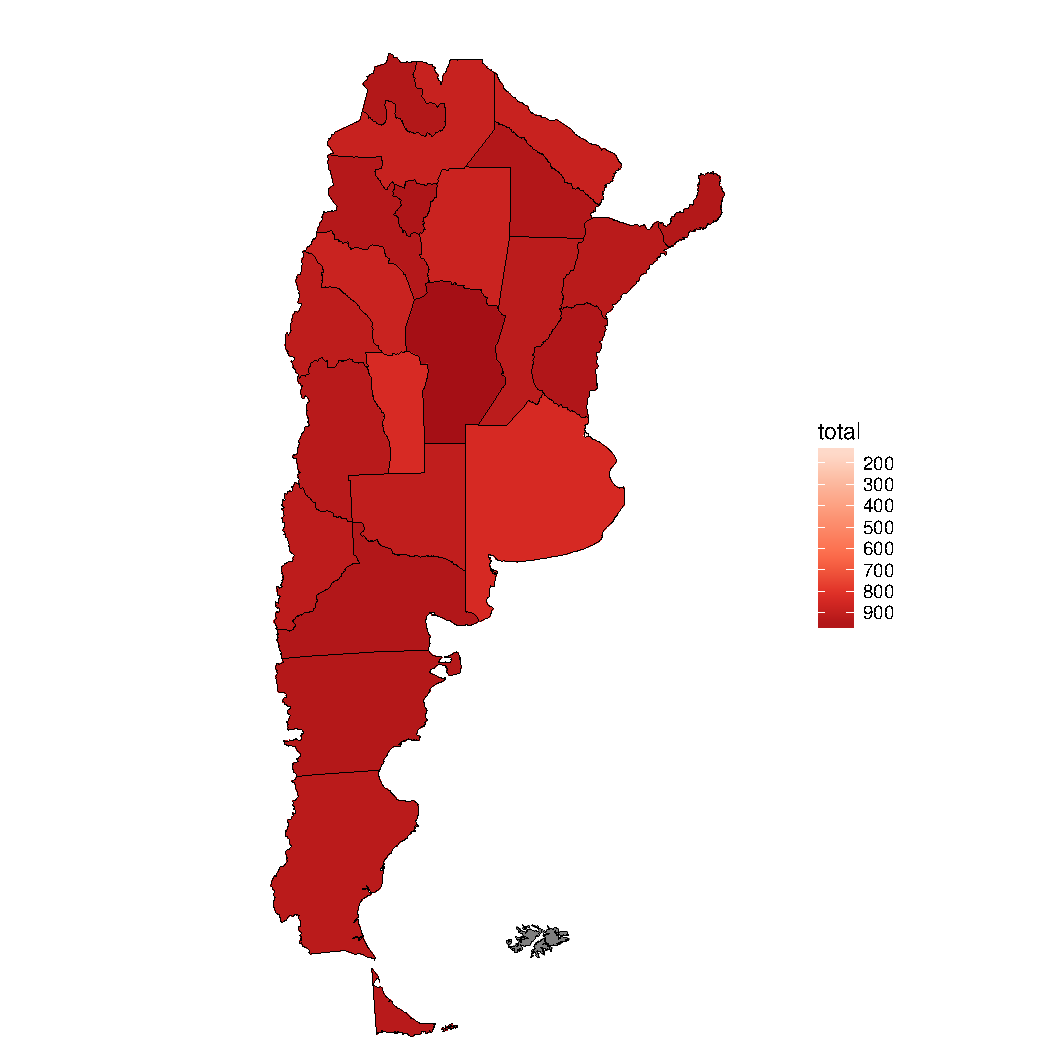
\includegraphics[width=\linewidth]{./images/mapaprovincias.pdf}
    \caption{} 
    \label{fig:mapaProvincias} 
   \end{minipage}
   \begin{minipage}[t]{0.31\textwidth}
    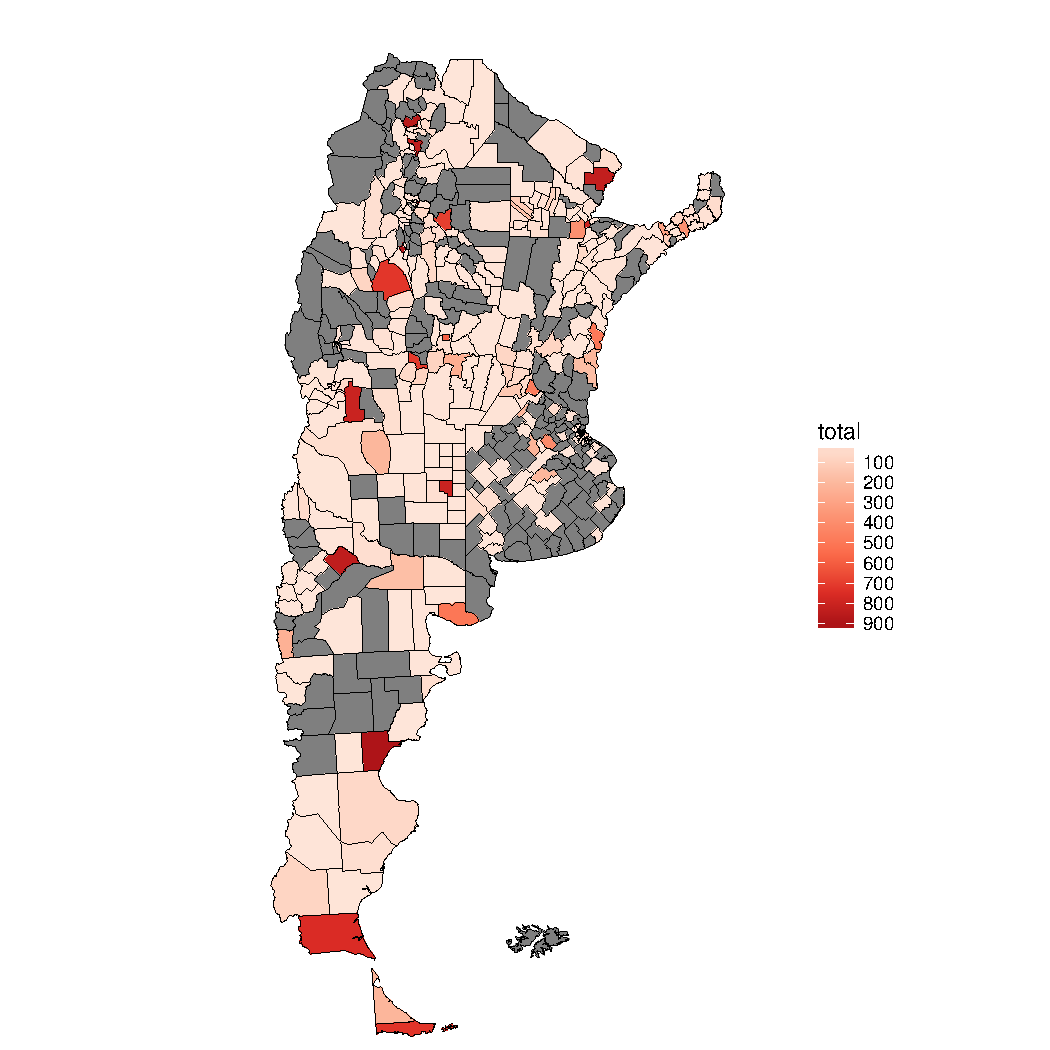
\includegraphics[width=\linewidth]{./images/mapadepartamentos.pdf}
    \caption{} 
    \label{fig:mapaDepartamentos} 
   \end{minipage}
   \begin{minipage}[t]{0.31\textwidth}
    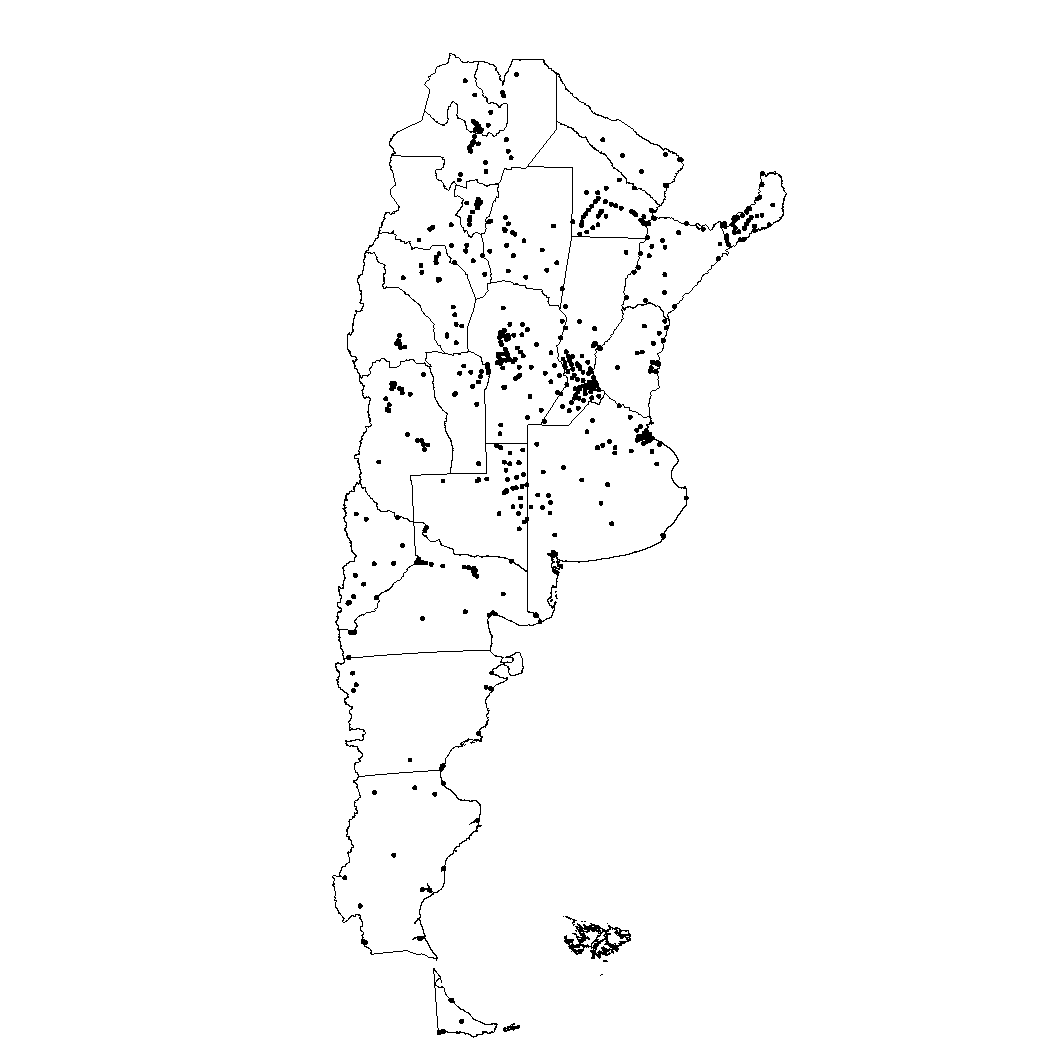
\includegraphics[width=\linewidth]{./images/mapaprovinciasConPuntos.pdf}
    \caption{} 
    \label{fig:mapaPuntos} 
   \end{minipage}
   



   \caption{Ubicaciones de los usuarios: En la figura \ref{fig:mapaProvincias} se muestra un mapa de Argentina con la distribución de los usuarios en las provincias sobre el conjunto de desarrollo. El mapa de la figura \ref{fig:mapaDepartamentos} permite visualizar la distribución de los usuarios en los departamentos sobre el conjunto de desarrollo. Se muestra con áreas grises los departamentos que no poseen usuarios que hayan definido el campo ubicación de su perfil en ese lugar. El mapa \ref{fig:mapaPuntos} muestra la distribución de las coordenadas obtenidas a partir de todos los usuarios del conjunto de desarrollo. Las coordenadas fueron obtenidas a través de un proceso de geocodificación. } 
  \label{fig:busqueda_usuarios} 

\end{figure}

En la figura \ref{fig:mapaProvincias} podemos observar que los usuarios que obtuvimos en las búsquedas se distribuyen de manera uniforme a través de las provincias. Si bien en la figura \ref{fig:mapaDepartamentos} hay regiones grises que indican la ausencia de usuarios en ese lugar, cabe destacar que los mapas se realizaron obteniendo las coordenadas geográficas a partir de la ubicación definida en el perfil del usuario. Por lo tanto, si una persona declara que vive en \textit{Tucumán, Argentina}, contabilizamos como que esa persona vive en la capital de esa provincia, lo cual puede no ser cierto. Sin embargo, esto no invalida los resultados puesto que la granularidad del análisis es a nivel provincial. Finalmente para ver la distribución de las coordenadas de los usuarios a lo largo del país mostramos la figura \ref{fig:mapaPuntos}. Se puede observar que en la mayoría de las grandes ciudades hay usuarios en nuestro conjunto de datos. Podemos observar en la figura \ref{fig:mapaGPS} del apéndice un mapa donde se contabilizaron todos los tuits con coordenadas geográficas del conjunto de datos. En este gráfico se puede observar que la distribución es mucho más amplia, aunque sigue habiendo más concentración de usuarios en aquellos departamentos con más densidad poblacional.

% \section{Datos de desarrollo y de validación}

% Por cada provincia se tomó a los usuarios de la misma y se los dividió para tener un conjunto de datos de desarrollo y uno de validación. El conjunto de validación fue creado para poder corroborar que los resultados obtenidos por el análisis del conjunto de desarrollo no sean algo intrínseco de esta muestra, sino que se pueden extrapolar a toda la población. 
% La división de los datos se realizó de manera tal que los conjuntos resultantes sean lo más independientes posibles: 
% \begin{description}
%     \item [Usuarios disjuntos] Debido a que ciertos usuarios repiten palabras constantemente, ya sea porque son bots o simplemente porque hablan siempre de los mismos temas, es adecuado validar los resultados con textos producidos por distintos usuarios. De esta manera se intentó mitigar el ruido generado por estos usuarios particulares.
%     \item [Fechas disjuntas] Al analizar los resultados sobre los textos generados en un tiempo acotado de tiempo, estamos trabajando con una muestra específica que es de esperar que tenga fenómenos particulares debido al momento en que fueron escritos. Por ejemplo, debido a cierto fenómeno climático o en el transcurso de un evento polémico (como un debate presidencial o un torneo deportivo), se pueden obtener tuits con una frecuencia de ciertas palabras muy distinta a la frecuencia que tiene normalmente. Por esta razón se dividieron los tuits producidos por los usuarios de manera tal que sus fechas sean disjuntas.
% \end{description}

% La división fue de la siguiente manera:
% Sobre el conjunto de usuarios se dividió en dos de forma aleatoria, con lo que se obtuvo $Usuarios_1$ y $Usuarios_2$. Luego se buscó la fecha $Fecha_{DIV}$ por la cual había una cantidad equiparable entre el conjunto de tuits producidos por  $Usuarios_1$ antes de $Fecha_{DIV}$ y el conjunto de tuits producidos por $Usuarios_2$ después de $Fecha_{DIV}$. Para encontrar la fecha se hizo una búsqueda binaria: dada una fecha $Fecha_{temp}$ (inicialmente es el día intermedio entre la fecha del primer y último tuit recolectado) se calcula la cantidad de tuits que hay con fechas anteriores sobre el conjunto de usuarios $Usuarios_1$ y análogamente se calcula la cantidad de tuits posteriores a esa fecha sobre el otro conjunto de usuarios. Si la cantidad del primer conjunto de tuits es menor que la del segundo conjunto, la $Fecha_{DIV}$ se busca en  el intervalo [$Fecha_{temp}-FechaFinal$] y se repite el procedimiento. Por lo tanto se cumple la siguiente ecuación:

% \begin{equation}
% %\sum_{ f = FechaInicial}^{Fecha_{Div}} tweets(Usuarios_1,f) \approx \sum_{ f = Fecha_{Div}}^{FechaFinal} tweets(Usuarios_2,f) 
%  Fecha_{DIV}  = \operatorname*{arg\,min}_{F} \left|\sum_{ f = FechaInicial}^{F} tuits(Usuarios_1,f) - \sum_{ f = F}^{FechaFinal} tuits(Usuarios_2,f)\right|
% \end{equation}
% Donde $FechaInicial$ es la fecha del primer tuit recolectado  y $FechaFinal$ es la del último.\\

% Después de fijar la fecha se dividió el conjunto de tuits producidos por estos usuarios: el conjunto de desarrollo con los tuits producidos antes de $Fecha_{DIV}$ y el conjunto de test producidos posteriormente a esa fecha.

\section{Tokenización y normalización}

En cuanto al análisis del texto surge una primer problemática: ¿qué es una palabra? En principio podemos definir a una palabra como cualquier secuencia de caracteres delimitados por espacios blancos. Con esta definición \textit{523456} y \textit{?} serían palabras. Debido a esto podríamos restringir nuestra definición a una secuencia de caracteres alfabéticos. Los ejemplos mencionados anteriormente dejarían de estar dentro de la definición. Sin embargo términos como \textit{asdsdafsdf} también serían palabras. Para evitar este problema podríamos tener un diccionario como filtro para saber si una secuencia de caracteres dada es una palabra. Si bien esto tendría mucha precisión al momento de filtrar los términos, no sería capaz de detectar palabras que existen en una lengua pero que no están incluidos en el diccionario elegido. Además, dada la cantidad de palabras recogidas, es altamente improbable que una secuencia al azar de caracteres alfabéticos reúna las condiciones de frecuencia necesarias para resultar destacada por la métrica que utilizamos. Es por eso que decidimos tomar a una palabra como una secuencia de caracteres alfabéticos.

Es muy posible que tengamos palabras que no sean interesantes a nivel lingüístico, como errores de tipeo (e.g computadira, escribur), errores ortográficos o  nombres propios. Es importante destacar que Twitter tiene caracteres especiales para mencionar a la gente, como el @, o el \#(hashtag) utilizado para agrupar mensajes. Estos caracteres aparecen mucho, ya que los usuarios suelen responderse en la red, mencionando los mismos temas (aclarando el hashtag), o respondiendo a otros usuarios. Ya que esos caracteres no son alfabéticos, cualquier término que los utilice no va a ser parte del conjunto de palabras, como tampoco lo serán las direcciones de páginas web. Decidimos que se filtren estos términos ya que no tienen interés lingüístico y además agregarían mucho ruido a los datos.

Además de la tokenización del texto, se realizó una normalización sobre él. Todas las letras se convirtieron a letra minúscula y las palabras con más de tres letras iguales de forma consecutiva se redujeron para que solo tengan tres repeticiones. De esta forma, el término \textit{padreeeee} y \textit{padreeee} fueron reducidos a una única unidad léxica (\textit{padreee}). Esto se hizo con la librería \textit{TweetTokenizer de NLTK}. 
Se descartó la idea de filtrar las palabras que no estuvieran en un diccionario ya que si bien hubiera eliminado mucho ruido, también nos hubiera filtrado palabras de interés. Este es el caso de los neologismos, o las palabras que, si bien se utilizan hace mucho tiempo, no están en los diccionarios actuales.

\section{Caracterización de la muestra}

Para tener una noción más completa de la muestra, se presenta la tabla \ref{tab:cantidades} que indica las cantidades de palabras y tuits por provincia.


\begin{table}[ht]
\centering


\begin{tabular}[width=0.7\textwidth]{|l|c|c|c|c|c|c|}
\hline
Provincia      & \#Palabras Distintas & \#Usuarios & \#Tuits & \#Total Palabras \\ \hline
Buenos Aires   & 191919       & 920          & 1125042    & 8974372  \\
Catamarca      & 173104       & 957          & 1057019    & 8161309   \\
Chaco          & 169476       & 964          & 976943     & 7605991   \\
Chubut         & 182592       & 954          & 1023373    & 8884745   \\
Córdoba        & 207307       & 987          & 1224266    & 10075932  \\
Corrientes     & 183292       & 939          & 1044951    & 8426940   \\
Entre Ríos     & 188679       & 969          & 1193693    & 9462986  \\
Formosa        & 169254       & 903          & 923352     & 7184382   \\
Jujuy          & 171064       & 971          & 678004     & 5951778   \\
La Pampa       & 186593       & 935          & 1085757    & 8996318  \\
La Rioja       & 186041       & 946          & 704044     & 6757277  \\
Mendoza        & 193708       & 945          & 1099717    & 9402399   \\
Misiones       & 168400       & 972          & 984218     & 7790197   \\
Neuquén        & 188038       & 927          & 1111201    & 9021449   \\
Río Negro      & 194383       & 965          & 1215361    & 9991831  \\
Salta          & 188402       & 884          & 830916     & 7506652   \\
San Juan       & 183546       & 926          & 1002322    & 8377792  \\
San Luis       & 164185       & 896          & 1006464    & 8327093  \\
Santa Cruz     & 174089       & 935          & 876621     & 7432923  \\
Santa Fe       & 201879       & 937          & 1019620    & 8862328  \\
Santiago del Estero       & 166540       & 887          & 944109     & 7355729  \\
Tierra del Fuego & 197273       & 964          & 976426     & 8559218   \\
Tucumán        & 195643       & 962          & 1093874    & 9238526 \\
  \hline
\end{tabular}
\caption{Cantidades del conjunto de datos}
\label{tab:cantidades}
\end{table}



También analizamos la cantidad de palabras por tuit promediadas sobre cada usuario.
Debido a que los tuits están limitados a 140 caracteres, era de esperar que no hubieran demasiadas palabras promedio por cada tuit. En la figura \ref{fig:cantPalabrasUsuario} podemos observar que la media para la cantidad de palabras promedio en un tuit está entre 7 y 8.
\begin{figure}[!ht]\centering
  \begin{minipage}[t]{0.49\textwidth}
    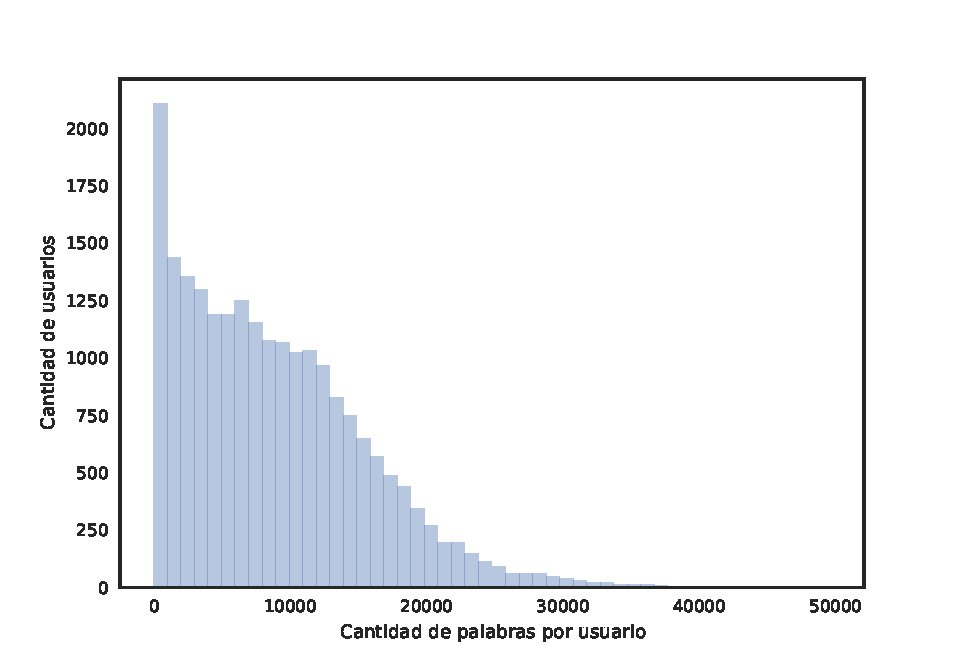
\includegraphics[width=\linewidth]{images2/cantPalabrasUsuario_sinFiltro.pdf}
    \caption{Histograma de la cantidad de palabras totales por cada usuario.} 
    \label{fig:cantPalabrasUsuario} 
   \end{minipage}
   \begin{minipage}[t]{0.49\textwidth}
    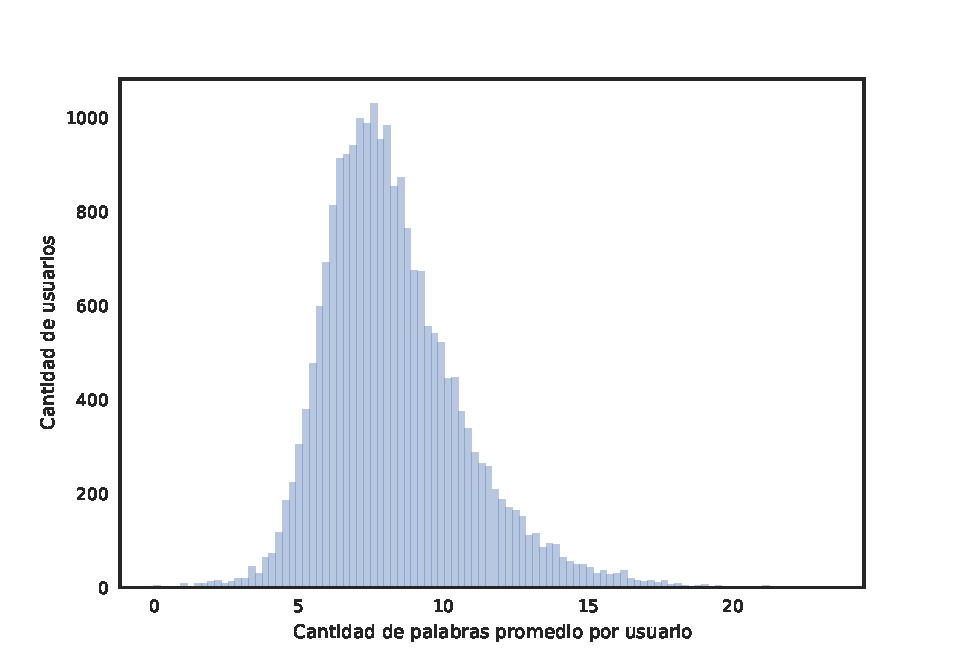
\includegraphics[width=\linewidth]{images2/cantPalabrasPromedio_sinFiltro.pdf}
    \caption{Histograma de la cantidad de palabras promedio para todos los usuarios.} 
    \label{fig:cantPalabrasPromedio} 
   \end{minipage}
   
\end{figure}

%Cantidad de palabras promedio por tweet
%Cantidad de palabras por usuario + varianza por provincia
\subsection{Distribución temporal de tuits}
Los tuits recolectados para el conjunto de datos de desarrollo tienen una particularidad: la cantidad de tuits recolectados crece año a año. Esto se refleja en los gráficos de las figuras \ref{fig:histTweetsProvincia1} y \ref{fig:histTweetsProvincia2}.

\begin{figure}[!ht]\centering
   \begin{minipage}[t]{0.49\textwidth}
     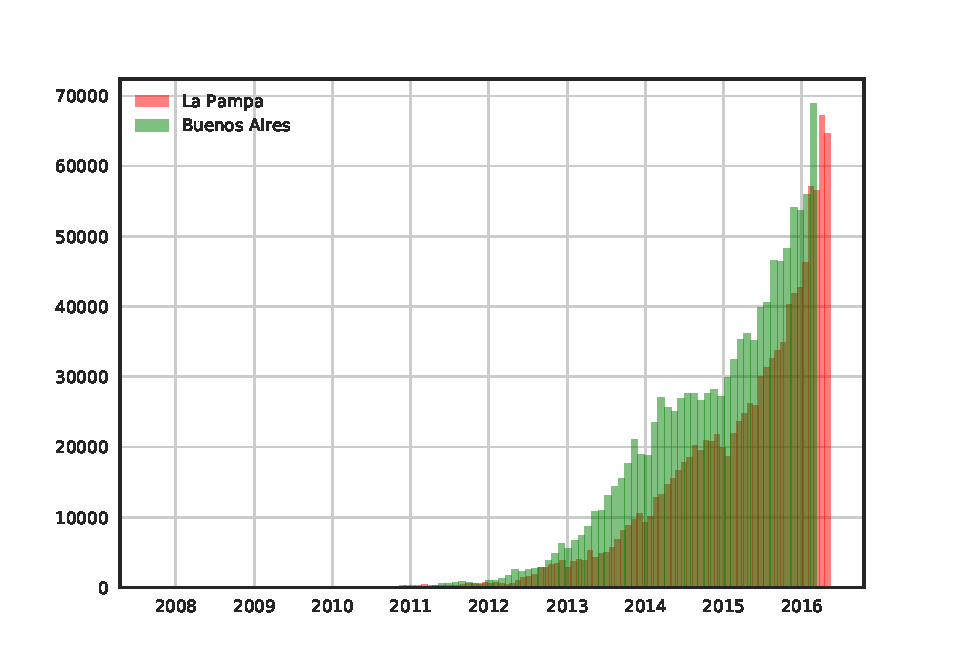
\includegraphics[width=\linewidth]{images2/histTweetsProvincia1_sinFiltro.pdf}
     \caption{}
     \label{fig:histTweetsProvincia1}
   \end{minipage}
   \begin {minipage}[t]{0.49\textwidth}
     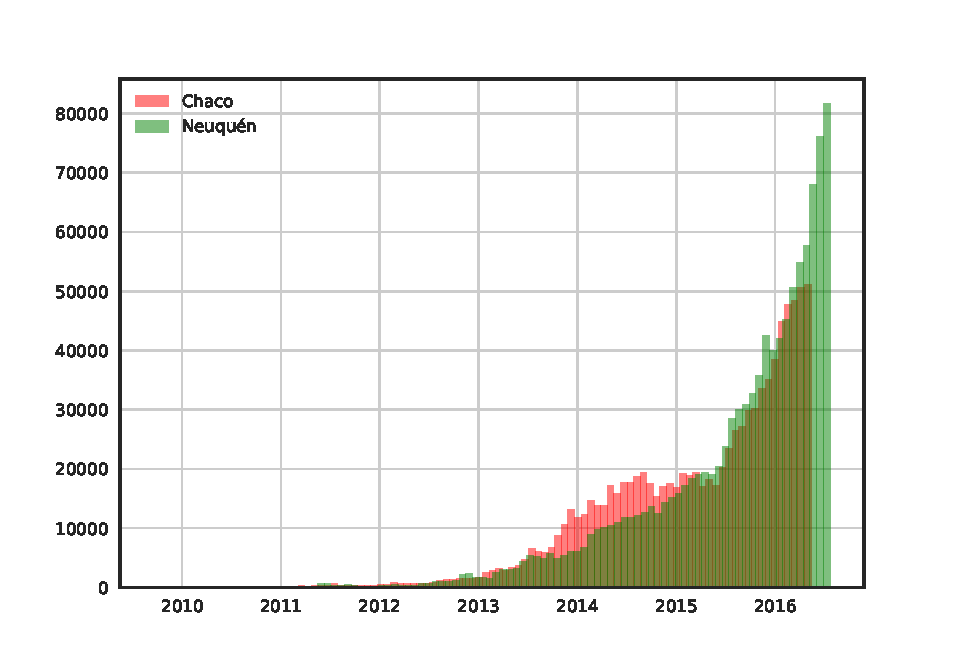
\includegraphics[width=\linewidth]{images2/histTweetsProvincia2_sinFiltro.pdf}
     \caption{}
     \label{fig:histTweetsProvincia2}
   \end{minipage}
   \caption { En la figura \ref{fig:histTweetsProvincia1} se presenta un histograma donde se muestra la cantidad de tuits que se hicieron por intervalo de tiempo en la provincias La Pampa y Buenos Aires. En la figura \ref{fig:histTweetsProvincia2}, se presenta el gráfico para Chaco y Neuquén.}
\end{figure}


% Tweets promedio por usuario, por provincia. (varianza)

% cantidad de tweets por usuario, cantidad media de palabras por usuario